\chapter{Scanning post Heavy Water Loading}
\label{Chap:D2O}

\section{Introduction}

\subsection{Heavy Water Uses}

When most people think of \ac{D$_2$O} they usually think of the the production of nuclear energy and atomic weaponry. However, a very important use of heavy water now is as an isotopic tracer in studies of biochemical processes, such as the assessment of body composition \cite{INTERNATIONALATOMICENERGYAGENCY2011IntroductionSpectrometry} and it is now also often being used to study triglyceride \cite{Strawford2004AdiposeO} and lipid turnover \cite{Wilkinson2017StableFuture}. Studies of lipogenesis in the liver are performed to investigate characteristics of liver disease \cite{Turner2003MeasurementMIDA}. This often involves giving study participants heavy water for a long period of time and then taking blood or tissue samples and analysing them \textit{in vitro} using mass spectrometry \cite{Lawitz2022ElevatedPatients, Diraison1997MeasuringTechniques}. The need for invasive sampling leads to limits on how many measurements can be taken and from where they can be taken, in order to avoid patient discomfort. Deuterium magnetic resonance could potentially offer a way to characterise and investigate liver disease non-invasively. 

After drinking \ac{D$_2$O}, rapid exchange occurs between exchangeable hydrogen atoms and deuterium atoms. This produces an increase in the concentration of \ac{HDO} from that present at natural abundance (NA). This consequently produces an increase in the strength of the \ac{NMR} from $^2$H in water. Covalently bonded hydrogens that exist in the methylene group (-CH$_2$) of fatty acids, can also potentially be replaced by deuterium atoms derived from heavy water, which causes the naturally abundant deuterated fat (CHD) signal to increase. More details on how $^2$H is incorporated into lipids and this increase in CHD signal can be found in Chapter \ref{Chap:Lipid}. Therefore by using \ac{CSI} over the liver whilst a participant/patient is loaded with heavy water and then tracking the change in concentration of fat/lipid signals over time, lipogenesis could in theory be studied. This approach could be useful in also studying general fat turnover not only in the liver but also in adipose and visceral fat as well. This sort of measurement was previously implemented in healthy and diabetic mice in the 1980's \cite{Brereton1986PreliminarySpectroscopy,Brereton1989TheMice}.

% Removed ', this exchange also occurs with' between increase and Covalent
\subsection{Relaxation Times}

\Ac{DMI} has been shown to be able to provide spatially resolved measurements of metabolite concentrations \cite{Kreis2020MeasuringMRI,Lu2017QuantitativeSpectroscopy}. This makes \ac{DMI} of clinical importance, as the metabolite concentrations could potentially be used as bio-markers to assess metabolic disease or tumour aggressiveness, on a patient-to-patient basis. It is straightforward to compare the strengths of different metabolite signals, but to work out absolute concentrations you need a reference and also need to account for the effects of relaxation on the signal strengths. 
% Simply you can calculate molecular abundance by comparing the MR signal of a known abundance to the MR signal of an unknown enrichment, however calculating absolute concentration is more complicated. 

In \ac{DMI} this is performed by comparing the naturally abundant MR signal of \ac{HDO} to the MR signal of other metabolites, along with an attenuation factor which is based on the sequence used for signal acquisition along with the number of deuterium labels in the metabolite. An estimate of the concentration of \ac{HDO} at \ac{NA} ($\sim$0.015\%) in the brain is 12.6 mM. This is calculated by multiplying the number of moles in one litre of \ac{D$_2$O} (55.4 Mol) by the water fraction of the brain $\sim$73\% along with the \ac{NA} of $^2$H, remembering to take into account the two $^2$H labels.

The attenuation factor specifically depends on the \ac{TR}, flip angle ($\alpha$) and the T$_1$ of the metabolite in question. Consequently it is of great importance to have an understanding of how T$_1$ changes in different tissues. Proton relaxation times have previously been reported in the literature at multiple field strengths for different tissues in the brain \cite{Wright2008WaterOptimization}, and can be used for proton metabolite quantification. Previous measurements of \ac{HDO} relaxation times in human participants used non-localised data \cite{DeFeyter2018DeuteriumVivo, Ruhm2022Dynamic9.4T, Gursan2022ResidualMuscle} which means the variation of relaxation times across specific tissue compartments is not known, making tissue-specific metabolic concentration calculations difficult.  

\subsection{Aims}

$^2$H MRI at 7T was used to characterise the \ac{HDO} signals from the human brain in four healthy participants who increased their deuterated water content to $\sim$1.5\% over a six-week period by drinking \ac{D$_2$O}. The heavy water loading was carried out as part of a parallel study into immune cell proteomics. $^2$H MRI and MRS measurements were made on all four participants. This included \ac{MEGE} images acquired at a range of \ac{TR} values, from which T$_1$ and T$_2^*$ relaxation maps were calculated. Co-registration to higher resolution $^1$H images allowed T$_1$ and T$_2^*$ relaxation times of deuterium in \ac{HDO} in \ac{CSF}, \ac{GM}, and \ac{WM} to be reported. For two of the participants, $^2$H \ac{MRI}/\ac{MRS} data was also acquired during the initial $\sim$eight-hour loading period to track the time-course of $^2$H enrichment within the brain \cite{Cocking2023DeuteriumDosing}. The work described in this chapter formed the basis of the peer-reviewed paper `Deuterium brain imaging at 7T during D$_2$O dosing' published in the journal `Magnetic Resonance in Medicine' \cite{Cocking2023DeuteriumDosing}.

%When creating an MRS/MRI scan it is important to be aware of the transverse relaxation time (T$_{2}^{*}$) of the tissue and metabolite you are investigating as this gives excellent insight on to how the signal is decaying and allows you to choose appropriate TR's and $\alpha$'s for the scan.

\section{Methodology}

Six healthy participants in total took part in this $^2$H-imaging sub-study which was approved by the local institutional ethics committee and the volunteers gave informed consent. Two of the participants were scanned during a set-up phase in which we established the feasibility of $^2$H imaging and identified favourable imaging parameters. Here, I report data from four participants (A - D) who were subsequently scanned using the optimised imaging protocols. All scanning was performed on a 7T Philips Achieva scanner (Philips Healthcare, Amsterdam, The Netherlands), operating at 45.8 MHz for $^2$H and 298 MHz for $^1$H. A 26.4 cm inner diameter, dual-tuned $^1$H/$^2$H birdcage coil (Rapid Biomedical) was used for deuterium measurements, while the standard 32-channel Rx/2-channel Tx head coil (Nova Medical) was used for acquiring anatomical $^1$H images.  

The proteomics study required an initial loading regime in which the targeted enrichment was built up in around 8 hours. This was achieved by participants drinking between 12 and 16, $\sim$50 ml doses of 70\% D$_2$O/30\% H$_2$O every $\sim$30 minutes, with the total amount of \ac{D$_2$O} consumed adjusted according to the participant’s body weight, so that an enrichment of around 1.5\% was produced. The participants subsequently drank $\sim$50 ml of \ac{D$_2$O} each morning over the six-week study period to maintain a $\sim$1.5\% enrichment. Similar enrichment levels and durations have been used in recent studies \cite{Robinson2011Long-termSupplementation, Burger2017LeukemiaIbrutinib, Loomba2019DiscoveryLabeling} with no adverse events reported. However some participants experienced a brief period of dizziness during the initial loading phase due to the rapid rise in body water enrichment \cite{Robinson2011Long-termSupplementation}. 

% Not included as data not included: 'Saliva samples were also collected from participants at regular intervals during the study and analyzed using gas chromatography–mass spectrometry (GCMS)'\cite{Yang1998AssaySpectrometry}.  

\subsection{Initial Loading}

Two of the participants (A and B) were scanned during the initial 8-hour loading period to monitor the time-course of changes in the concentration of $^2$H in the brain. A scanning protocol of $\sim$15 minutes’ duration was performed before dosing and then again after 30, 90, 150, 210, 270, 360, 420 and 540 minutes. The protocol comprised, a $^1$H scout scan for planning, followed by acquisition of $^2$H pulse-acquire spectra from the whole head and then from a 2-cm-thick axial slice positioned over the lateral ventricles. Both used the following scan parameters: $\alpha$ = 90$^\circ$, 2048 samples, \ac{BW} = 3000 Hz, repetition time TR = 1 s and 64 averages (acquisition time T$_\text{scan}$ = 64 s). We then acquired axial, \ac{MEGE} $^2$H images (20 averages, T$_\text{scan}$ = 453s, \ac{FOV} = 288 $\times$ 288 $\times$ 80 mm$^3$, 6 $\times$ 6 $\times$ 10 mm$^3$ voxels, $\alpha$ = 33$^\circ$, \ac{TR} = 62 ms, five echoes, \ac{TE} = 8.9 ms and $\Delta$\ac{TE} = 8.4 ms. Axial $^1$H \ac{GE} images (T$_\text{scan}$ = 232 s, 32 slices, \ac{FOV} = 288 $\times$ 288 $\times$ 80 mm$^3$, 3 $\times$ 3 $\times$ 2.5 mm$^3$ voxels, \ac{TE} = 5.9 ms, \ac{TR} = 39 ms) were also acquired. The scanning protocol was repeated 17 days after the initial loading to obtain comparative data at steady-state enrichment. 

The spectroscopy measurements made before loading provided an estimate of the signal from naturally abundant deuterium in water: scaling subsequent measurements then allowed the absolute \ac{HDO} concentration to be estimated at each time-point. The \ac{HDO} concentration in the body was also estimated from the ratio of the total imbibed \ac{D$_2$O} volume to an estimate of total body water using the participant’s height, weight, age and gender \cite{Watson1980TotalMeasurements}. The temporal variation of \ac{HDO} concentration in the brain was monitored by plotting the amplitude of the single peak in each non-selective and selective spectrum against the time since the first heavy water dose. The peak amplitude was obtained by fitting the complex data to a Lorentzian line shape in the frequency domain using non-linear least squares fitting. 

\begin{figure}[H]
    \centering
    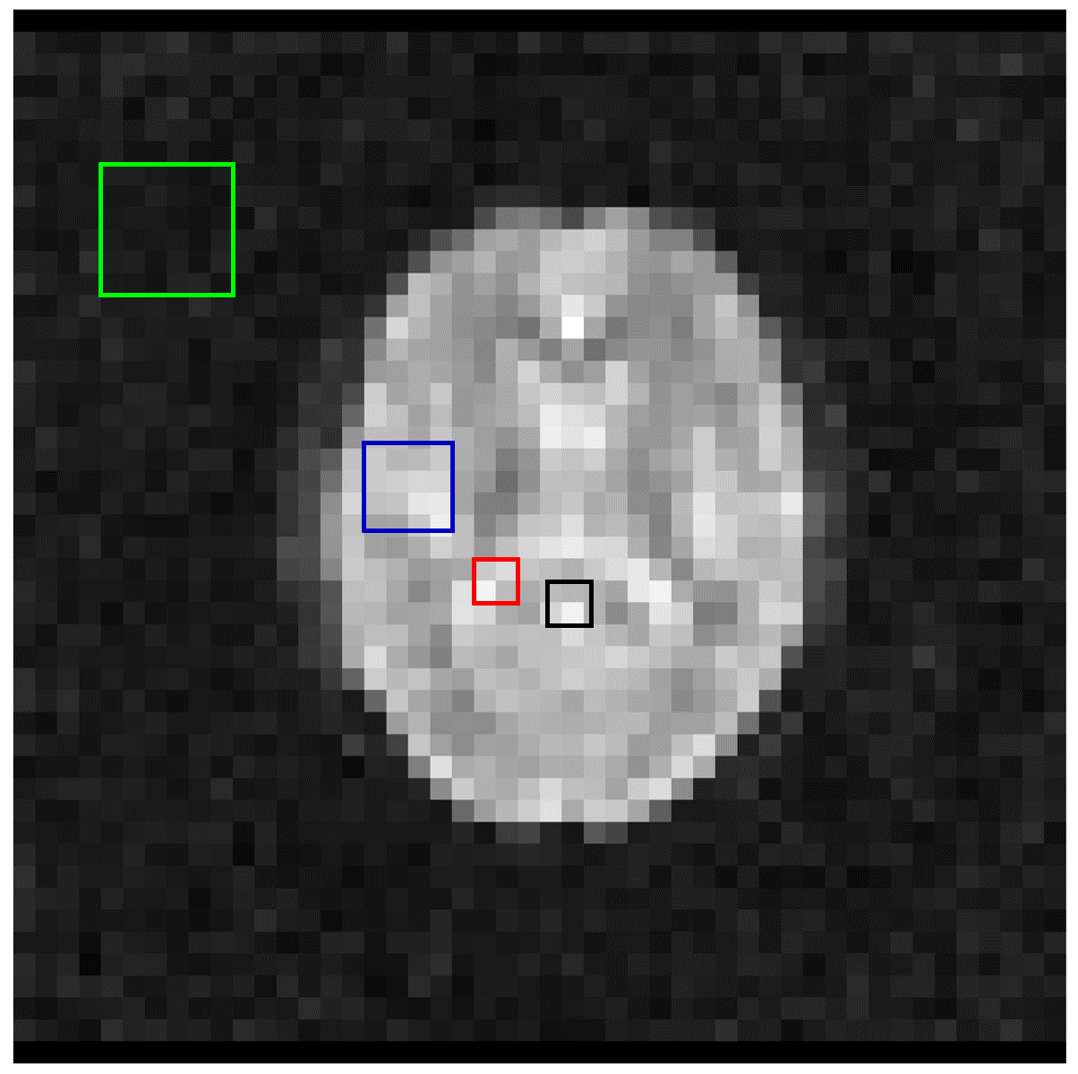
\includegraphics[width=0.7\textwidth]{Figures/D2O/ROI.png}
    \caption{\textit{Regions of interest used for following the time-course of signal change during \ac{D$_2$O} loading. Black = \ac{SC}; Red = lateral ventricle; Blue = brain (\ac{GM}, \ac{WM} and \ac{CSF}); Green = background noise.}}
    \label{fig:D2O:ROI}
\end{figure}

We used the image data to track the changes in $^2$H signal from different tissue compartments. The $^2$H images acquired at each time-point were summed over the five echoes to form a single image data set. Then using both the $^2$H and $^1$H images, regions of interest (ROI) were formed for a background region, general brain tissue, the lateral ventricles and for a region of high signal intensity thought to arise from blood vessels and \ac{CSF} in the superior cistern (SC). Examples of the \ac{ROI}s used are shown in Fig. \ref{fig:D2O:ROI}. The signal intensity in each region was plotted against time from the first heavy water dose. The \ac{SNR} in images acquired before loading was too low to make good estimates of \ac{NA} signal strength, so values were normalized to the signal measured in the superior cistern \ac{ROI} at the last time point of the initial loading period. All analysis was performed using MATLAB (Release 2020b, The MathWorks, Inc., Natick, MA, United States). Saliva samples were obtained and measured by gas chromatography–mass spectrometry (GCMS) from Participant A and B, as part of the parent project.

\subsection{Relaxation Time Measurements}
\label{Chap:D2O:Relaxation}

$^2$H relaxation times for water in \ac{CSF}, \ac{GM}, and \ac{WM} were calculated from data acquired during the six-week loading period using the dual-tuned $^2$H/$^1$H coils. In each imaging session, $^2$H 3D sagittal \ac{MEGE} images were acquired (voxels = 6 $\times$ 6 $\times$ 10 mm$^3$, \ac{FOV} = 288 $\times$ 288 $\times$ 240 mm$^3$, slices = 24) at a range of \ac{TR} values, along with $^1$H 3D \ac{MEGE} images (voxels = 3 $\times$ 3 $\times$ 5 mm$^3$, \ac{FOV} = 288 $\times$ 288 $\times$ 240 mm$^3$, slices = 48, 15 \ac{TE}s with TE$_1$ = 2.5 ms, $\Delta$TE = 2.34 ms, and TR = 41 ms). 

$^2$H \ac{MEGE} data from Participants A and B were acquired with five echoes (\ac{TE} = 4.3 ms, $\Delta$TE = 8.4 ms), $\alpha$ = 60° and \ac{TR} = 68, 136, 272 and 544 ms, with 8, 4, 2 and 1 averages so that T$_\text{scan}$ = 487 s for each image. $^2$H \ac{MEGE} data from participants C and D was acquired with six echoes (\ac{TE} = 4.3 ms; $\Delta$TE = 8.4 ms) and one additional \ac{TR} value (TR = 816 ms; T$_\text{scan}$ = 730 s; 1 average). 
The number of \ac{TE} and \ac{TR} values were increased for participants C and D to improve fitting quality. The $^2$H scanning sessions were performed twice on Participants C and D.

In a separate scanning session using the Nova coil, $^1$H  \ac{MPRAGE} images (0.7 mm resolution) and $^1$H 3D \ac{MEGE} images (3 $\times$ 3 $\times$ 5 mm$^3$ voxels, 15 echo times, TE$_1$ = 2.5 ms, $\Delta$TE = 2.57 ms, and \ac{TR} = 41 ms) were acquired from each participant. These images were used for image segmentation and estimation of the $^1$H T$_2^*$ values. 

For calculation of $^2$H relaxation time maps, we first estimated the variation of flip angle ($\alpha$) over the image volume by summing the images across \ac{TE}s, at each \ac{TR}, and then fitting the resulting image data voxel-wise to a saturation recovery curve (i.e., fitting signal variation with \ac{TR} for $\alpha$, R$_1$, and signal amplitude). The resulting flip-angle maps were smoothed by averaging over 5 $\times$ 5 $\times$ 5 voxel neighbourhood and the $\alpha$-values used as a fixed variable in dual-fitting the variation in signal intensity S$_{i,j}$ across TR$_i$ and TE$_j$  values. The absolute difference between the model and the obtained data was found and minimised, the mathematical form of this expression is given here  

\begin{equation}
     r = \sum_{i=1}^{n_{\text{TR}}}\sum_{j=1}^{n_{\text{TE}}}\left|\frac{A\sin{\alpha}(1-\exp(-R_1 \text{TR}_i)}{1-\cos{\alpha}\exp(-R_1 \text{TR}_i)}*\exp(-R_2^*\text{TE}_j) - S_{i,j}\right|^2
     \label{eqn.min}
\end{equation}

$r$ is the calculated value that is to be minimised. The Matlab fmincon command was used to perform the minimisation, $^1$H R$_2^*$ maps were obtained by similar fitting to the exponential signal decay with \ac{TE} in the $^1$H \ac{MEGE} data acquired using the Nova coil. The parameters and constraints used in the fmincon fitting are given in Table \ref{fig:D2O:fit}.

\begin{table}
    \centering
    
\includegraphics[width=0.7\linewidth]{Figures/D2O/Fit_Params.png}
    \caption{\textit{Parameters and constraints used in the Matlab fmincon fitting routines, (a) shows the parameters used to obtain the initial flip-angle ($\alpha$) map and (b) shows the parameters used in the main fitting routine to obtain relaxation rates. Average indicates the average of the masked brain image, and A$_\text{smooth}$ indicates the amplitude value from the smoothed map that was created after the flip-angle fitting.}}
    \label{fig:D2O:fit}
\end{table}

To evaluate the relaxation times in different compartments, we segmented the $^1$H \ac{MPRAGE} data using FSL FAST \cite{Zhang2001SegmentationAlgorithm} and transformed the resulting \ac{GM}, \ac{WM} and \ac{CSF} masks to the space of the $^2$H relaxation time maps. Following brain extraction using FSL BET \cite{Smith2002FastExtraction} and bias field correction, an affine matrix was obtained from image co-registration using FSL FLIRT \cite{Jenkinson2001AImages,Jenkinson2002ImprovedImages} which transformed the $^1$H \ac{MEGE} data acquired using the dual-tuned coil to the $^1$H \ac{MEGE} Nova Medical coil data, along with an affine matrix for the $^1$H \ac{MEGE} to \ac{MPRAGE} transformation. Image co-registration was linear, with six degrees of freedom and used the correlation ratio cost function \cite{RocheTheRegistration}. The \ac{MEGE} data were summed across echoes and repetition times before co-registration.

The brain-extracted \ac{MPRAGE} image was segmented to create binary masks for \ac{GM}, \ac{WM} and \ac{CSF} using FSL FAST \cite{Zhang2001SegmentationAlgorithm}. These masks were then transformed to the $^2$H space using the previously obtained affine matrices and the outer regions of the CSF mask were manually removed so that the majority of the CSF mask come from the lateral ventricles. The new masks were binarized at a value of 0.6 for each tissue to ensure that each mask contained at least 25 voxels for averaging. The binarized masks were applied to the relaxation maps for calculation of mean relaxation times for \ac{CSF}, \ac{GM} and \ac{WM}.

\section{Results}
\subsection{Loading}

\begin{figure}[H]
    \centering
    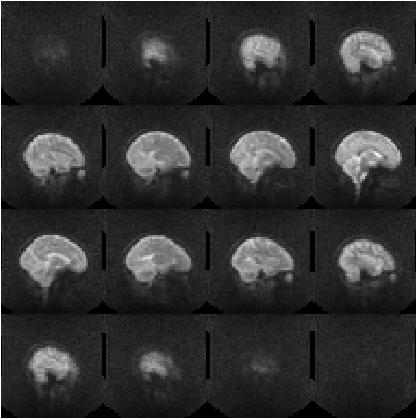
\includegraphics[width=0.7\textwidth]{Figures/D2O/Sag_Full.png}
    \caption{\textit{3D MEGE $^2$H image data from Participant C. Images produced by summing over six \ac{TE} values and five \ac{TR} values. Voxel size = 6 × 6 × 10 mm$^3$, in-plane \ac{FOV} = 288 × 288 mm$^2$, T$_\textrm{scan}=485$ s for each \ac{TR} value.}}
    \label{fig:D2O:Sag_Full}
\end{figure}

Figure \ref{fig:D2O:Sag_Full} shows example $^2$H 3D sagittal images obtained by summing the $^2$H \ac{MEGE} data for a single (fully loaded) subject over \ac{TE} and \ac{TR} values, during the steady-state loading period. The resulting images, which predominantly show T$_2^*$ contrast, clearly depict the brain anatomy and have a similar appearance to T$_2^*$-weighted, $^1$H images. The \ac{CSF} in the ventricles and at the cortical surface appears hyperintense, while regions of white matter where there is little partial-voluming with \ac{CSF}, such as in the corpus callosum, appear hypointense. Figure \ref{fig:D2O:TR_TE} shows the variation of image intensity with TE and TR in a central sagittal slice. The slower T$_2^*$ decay of the CSF signal compared with that of the \ac{GM} and \ac{WM} signals is evident, along with the signal saturation at reduced \ac{TR}, and the reduction of contrast at low \ac{TE} and \ac{TR} values. In Fig. \ref{fig:D2O:Load}, example $^2$H images acquired from participants A and B at different dosage times during the initial loading process are shown. As dosage increases, so does the overall \ac{SNR}. The \ac{ROI}s that were used to analyse the loading in different brain tissues are outlined in Fig. \ref{fig:D2O:ROI} (for participant A). Since the background \ac{MEGE} image is obtained after the final dose for Subject A the tissues being segmented are easily discerned in the $^2$H images. However, for the lower dosage images this is not the case, which is why the \ac{ROI}’s are defined on the anatomical $^1$H image. 

\begin{figure}[H]
    \centering
    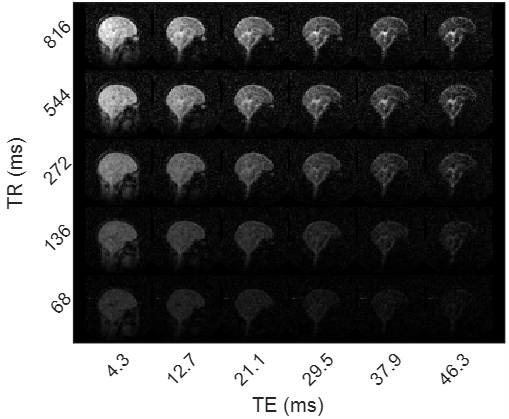
\includegraphics[width = 0.9\textwidth]{Figures/D2O/TR_TE.png}
    \caption{\textit{3D MEGE $^2$H image from one slice from Participant D. Images are displayed with TE value varying horizontally and TR-value varying vertically. Voxel size = 6 × 6 × 10 mm$^3$, in-plane FOV = 288 × 288 mm$^2$, T$_\textrm{scan} =$ 485 s for each \ac{TR} value.}}
    \label{fig:D2O:TR_TE}
\end{figure}

The qualitative increase in signal during the loading period in Fig. \ref{fig:D2O:Load} is shown more quantitatively in Fig. \ref{fig:D2O:Bulk}, which plots the $^2$H concentration time course obtained from the spectroscopy data, along with the steady-state values measured after 17 days of loading. The average signal from each \ac{ROI} during loading is shown in Fig. \ref{fig:D2O:ROI_Graph} scaled to the signal measured in the \ac{SC} at the last time point, in the brain along with the steady-state values measured after 17 days of loading. Plotted values from Figs. \ref{fig:D2O:Bulk} and \ref{fig:D2O:ROI_Graph} also show the $^2$H concentration estimated from the cumulative D$_2$O dose and estimated total body water volume, for comparison. The results from GCMS analysis of saliva samples are also plotted here for comparison.

\begin{figure}[H]
    \centering
    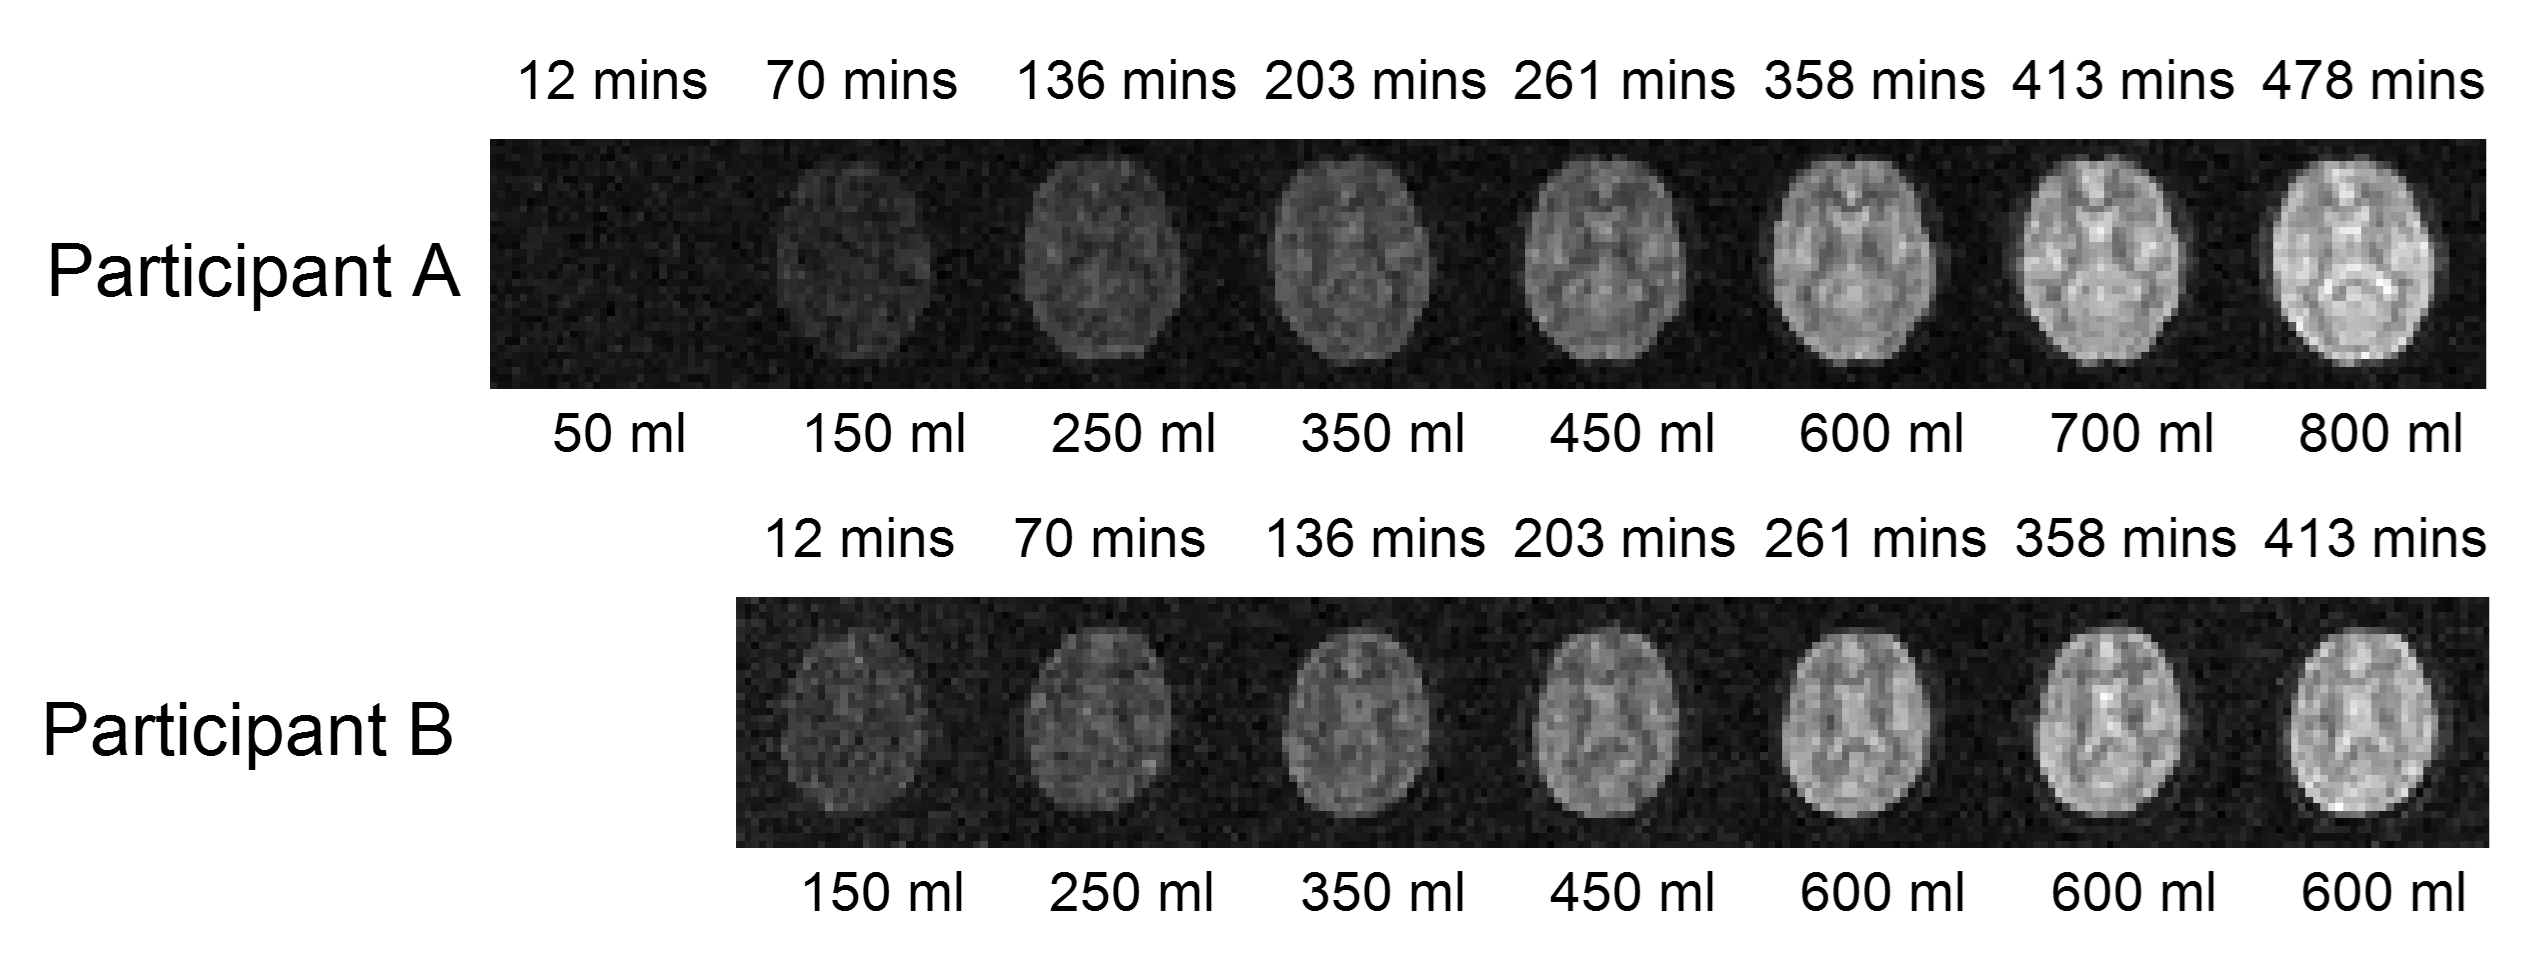
\includegraphics[width=1\textwidth]{Figures/D2O/Loading.png}
    \caption{\textit{$^2$H images acquired from two participants at different times during the initial, 8-hr heavy water loading period. The time since the first dose is indicated above each image and the cumulative dose of heavy water is indicated below. A single axial slice spanning the lateral ventricles is shown. The images shown are formed from the average over five echoes (TE$_1$ = 8.9 ms, $\Delta$TE = 8.4 ms) and have a reduced in-plane \ac{FOV} of 204 × 204 mm$^2$.}}
    \label{fig:D2O:Load}
\end{figure}

\subsection{Relaxation Times}

Figure \ref{fig:D2O:R1_R2} shows sagittal and axial relaxation rate maps from two participants, with the dominant feature in the $^2$H maps being the reduced R$_2^*$ and R$_1$ relaxation rates in the ventricles. The elevated R$_2^*$ values seen in deep grey matter structures in the $^1$H maps are not evident in the $^2$H maps. Scatter plots of the voxelwise T$_1$ and T$_2^*$ relaxation times and the proton and deuterium T$_2^*T$ relaxation times, across four subjects are shown in Fig. \ref{fig:D2O:scatter}. Table \ref{fig:D2O:R_times} reports the average and standard deviation of the $^2$H T$_1$ and T$_2^*$ values, along with $^1$H T$_2^*$ values measured measured in \ac{GM}, \ac{WM} and \ac{CSF} in the four participants. These values were calculated by applying the binarised segmentation masks to the relaxation maps.

\begin{figure}[H]
    \centering
    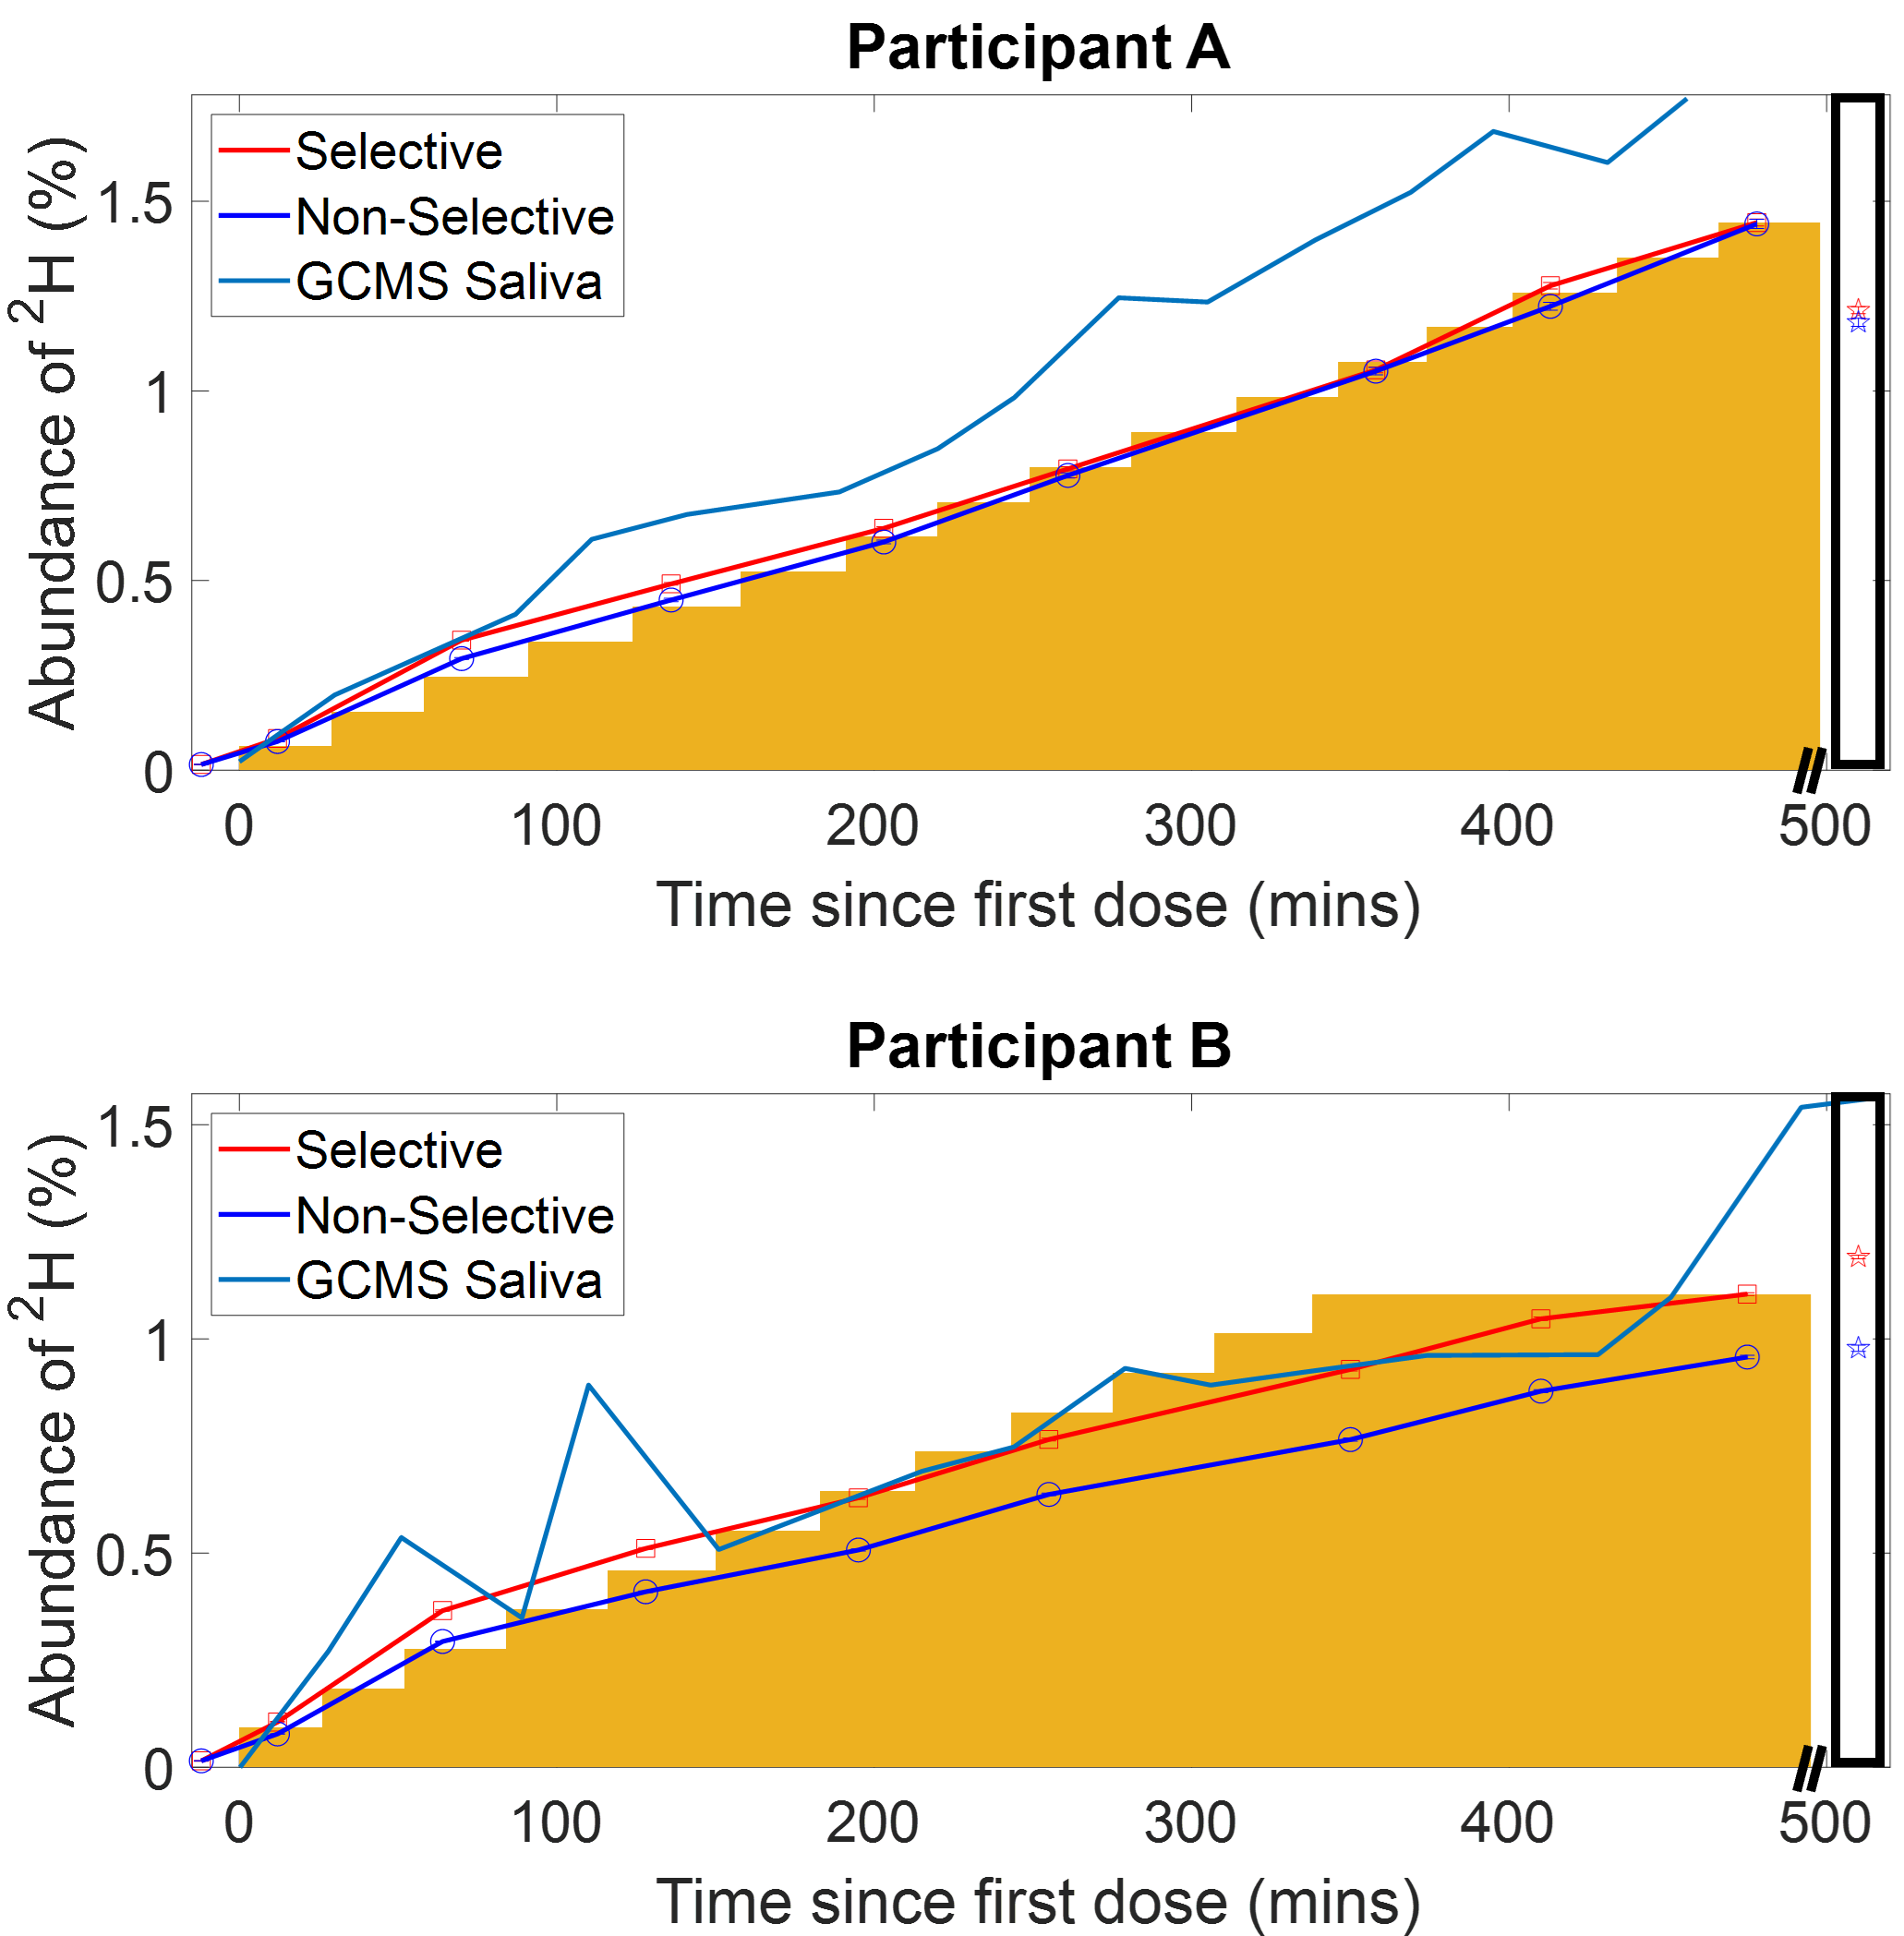
\includegraphics[width=1\textwidth]{Figures/D2O/Bulk_Graph.png}
    \caption{\textit{Time course of the concentration of deuterium in the brain estimated from the $^2$H spectroscopy measurements (red=from 2 cm slice at level of lateral ventricles; blue= whole head). Percentage estimated by scaling by the signal measured at \ac{NA} (assumed to be 0.015\%). The orange blocks indicate the concentration estimated from the cumulative D$_2$O dose and body weight. The measurements made at steady state (after 17 days of loading) are shown in the box at the far right. Measurements from saliva samples are given in the light-blue line.}}
    \label{fig:D2O:Bulk}
\end{figure}

\begin{figure}[H]
    \centering
    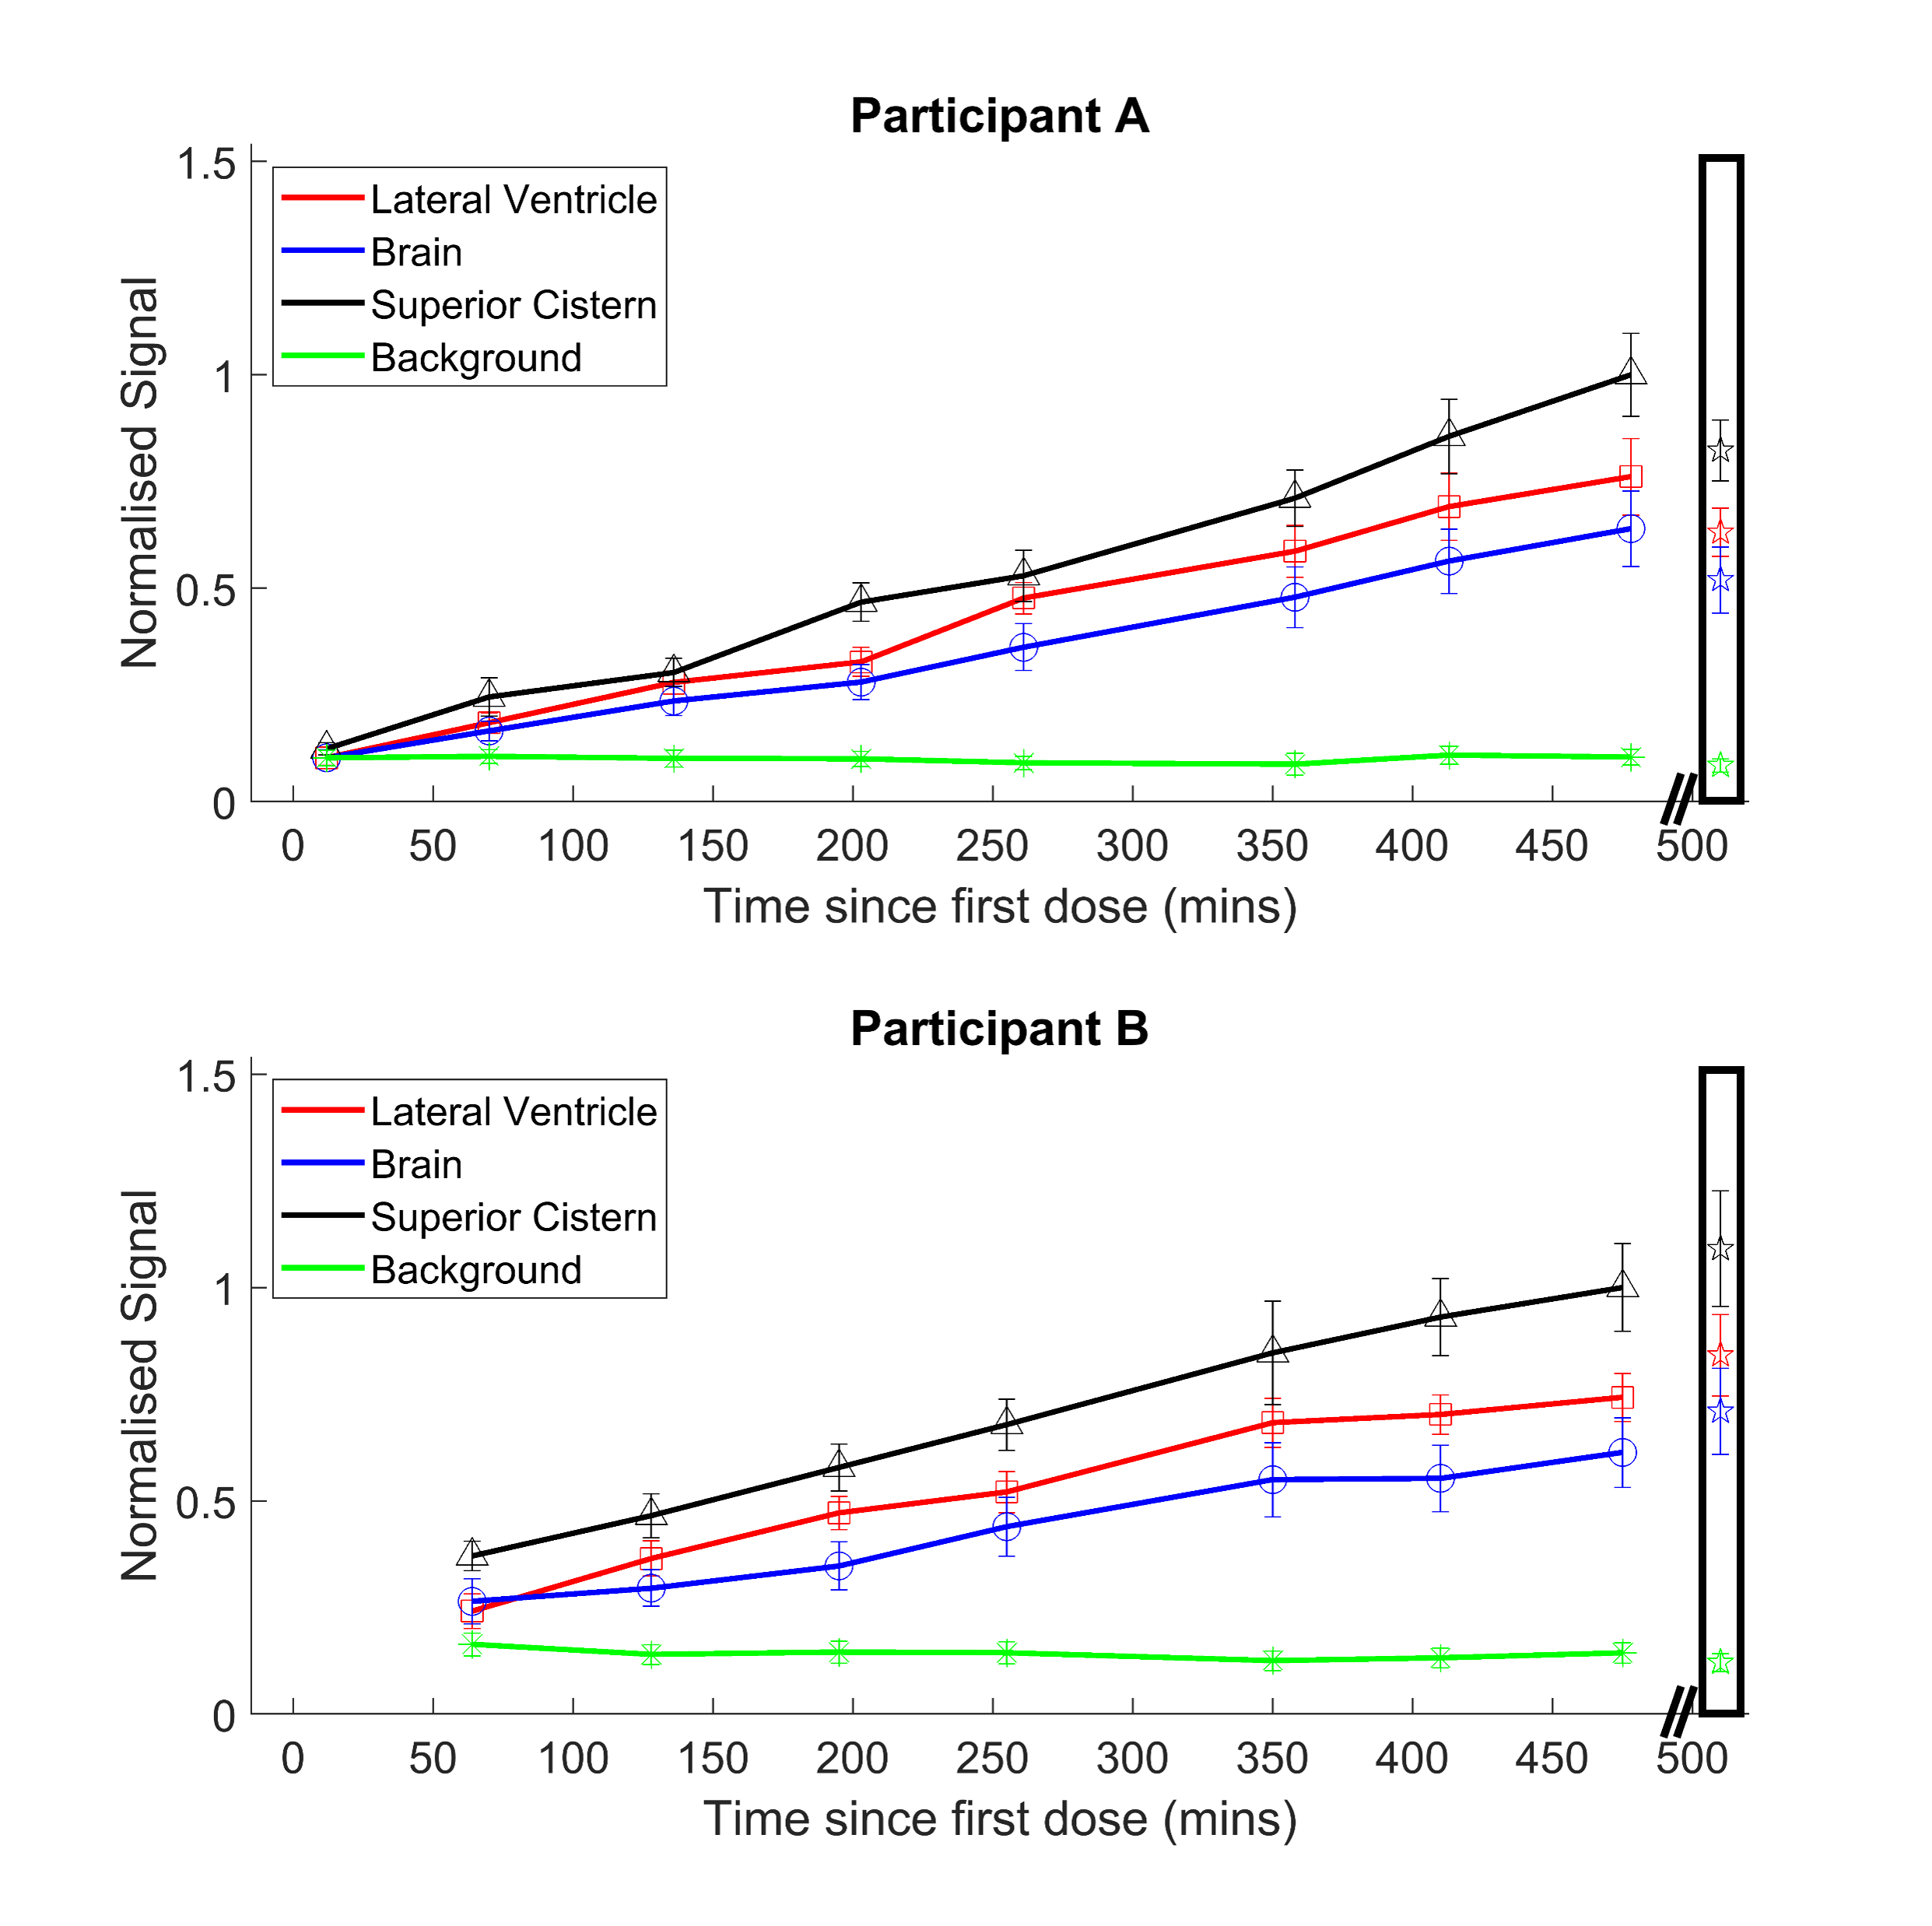
\includegraphics[width=1\textwidth]{Figures/D2O/ROI_Graph.png}
    \caption{\textit{Time course of average signal change in image ROIs (red=lateral ventricle; blue=brain tissue; black=\ac{SC}; green=background noise) in two participants. Signals from all compartments are scaled by the \ac{SC} signal at the final measurement time-point. Scaled signals measured at steady state (after 17-days loading) are shown in the box at the far right.}}
    \label{fig:D2O:ROI_Graph}
\end{figure}

\begin{figure}[H]
    \centering
    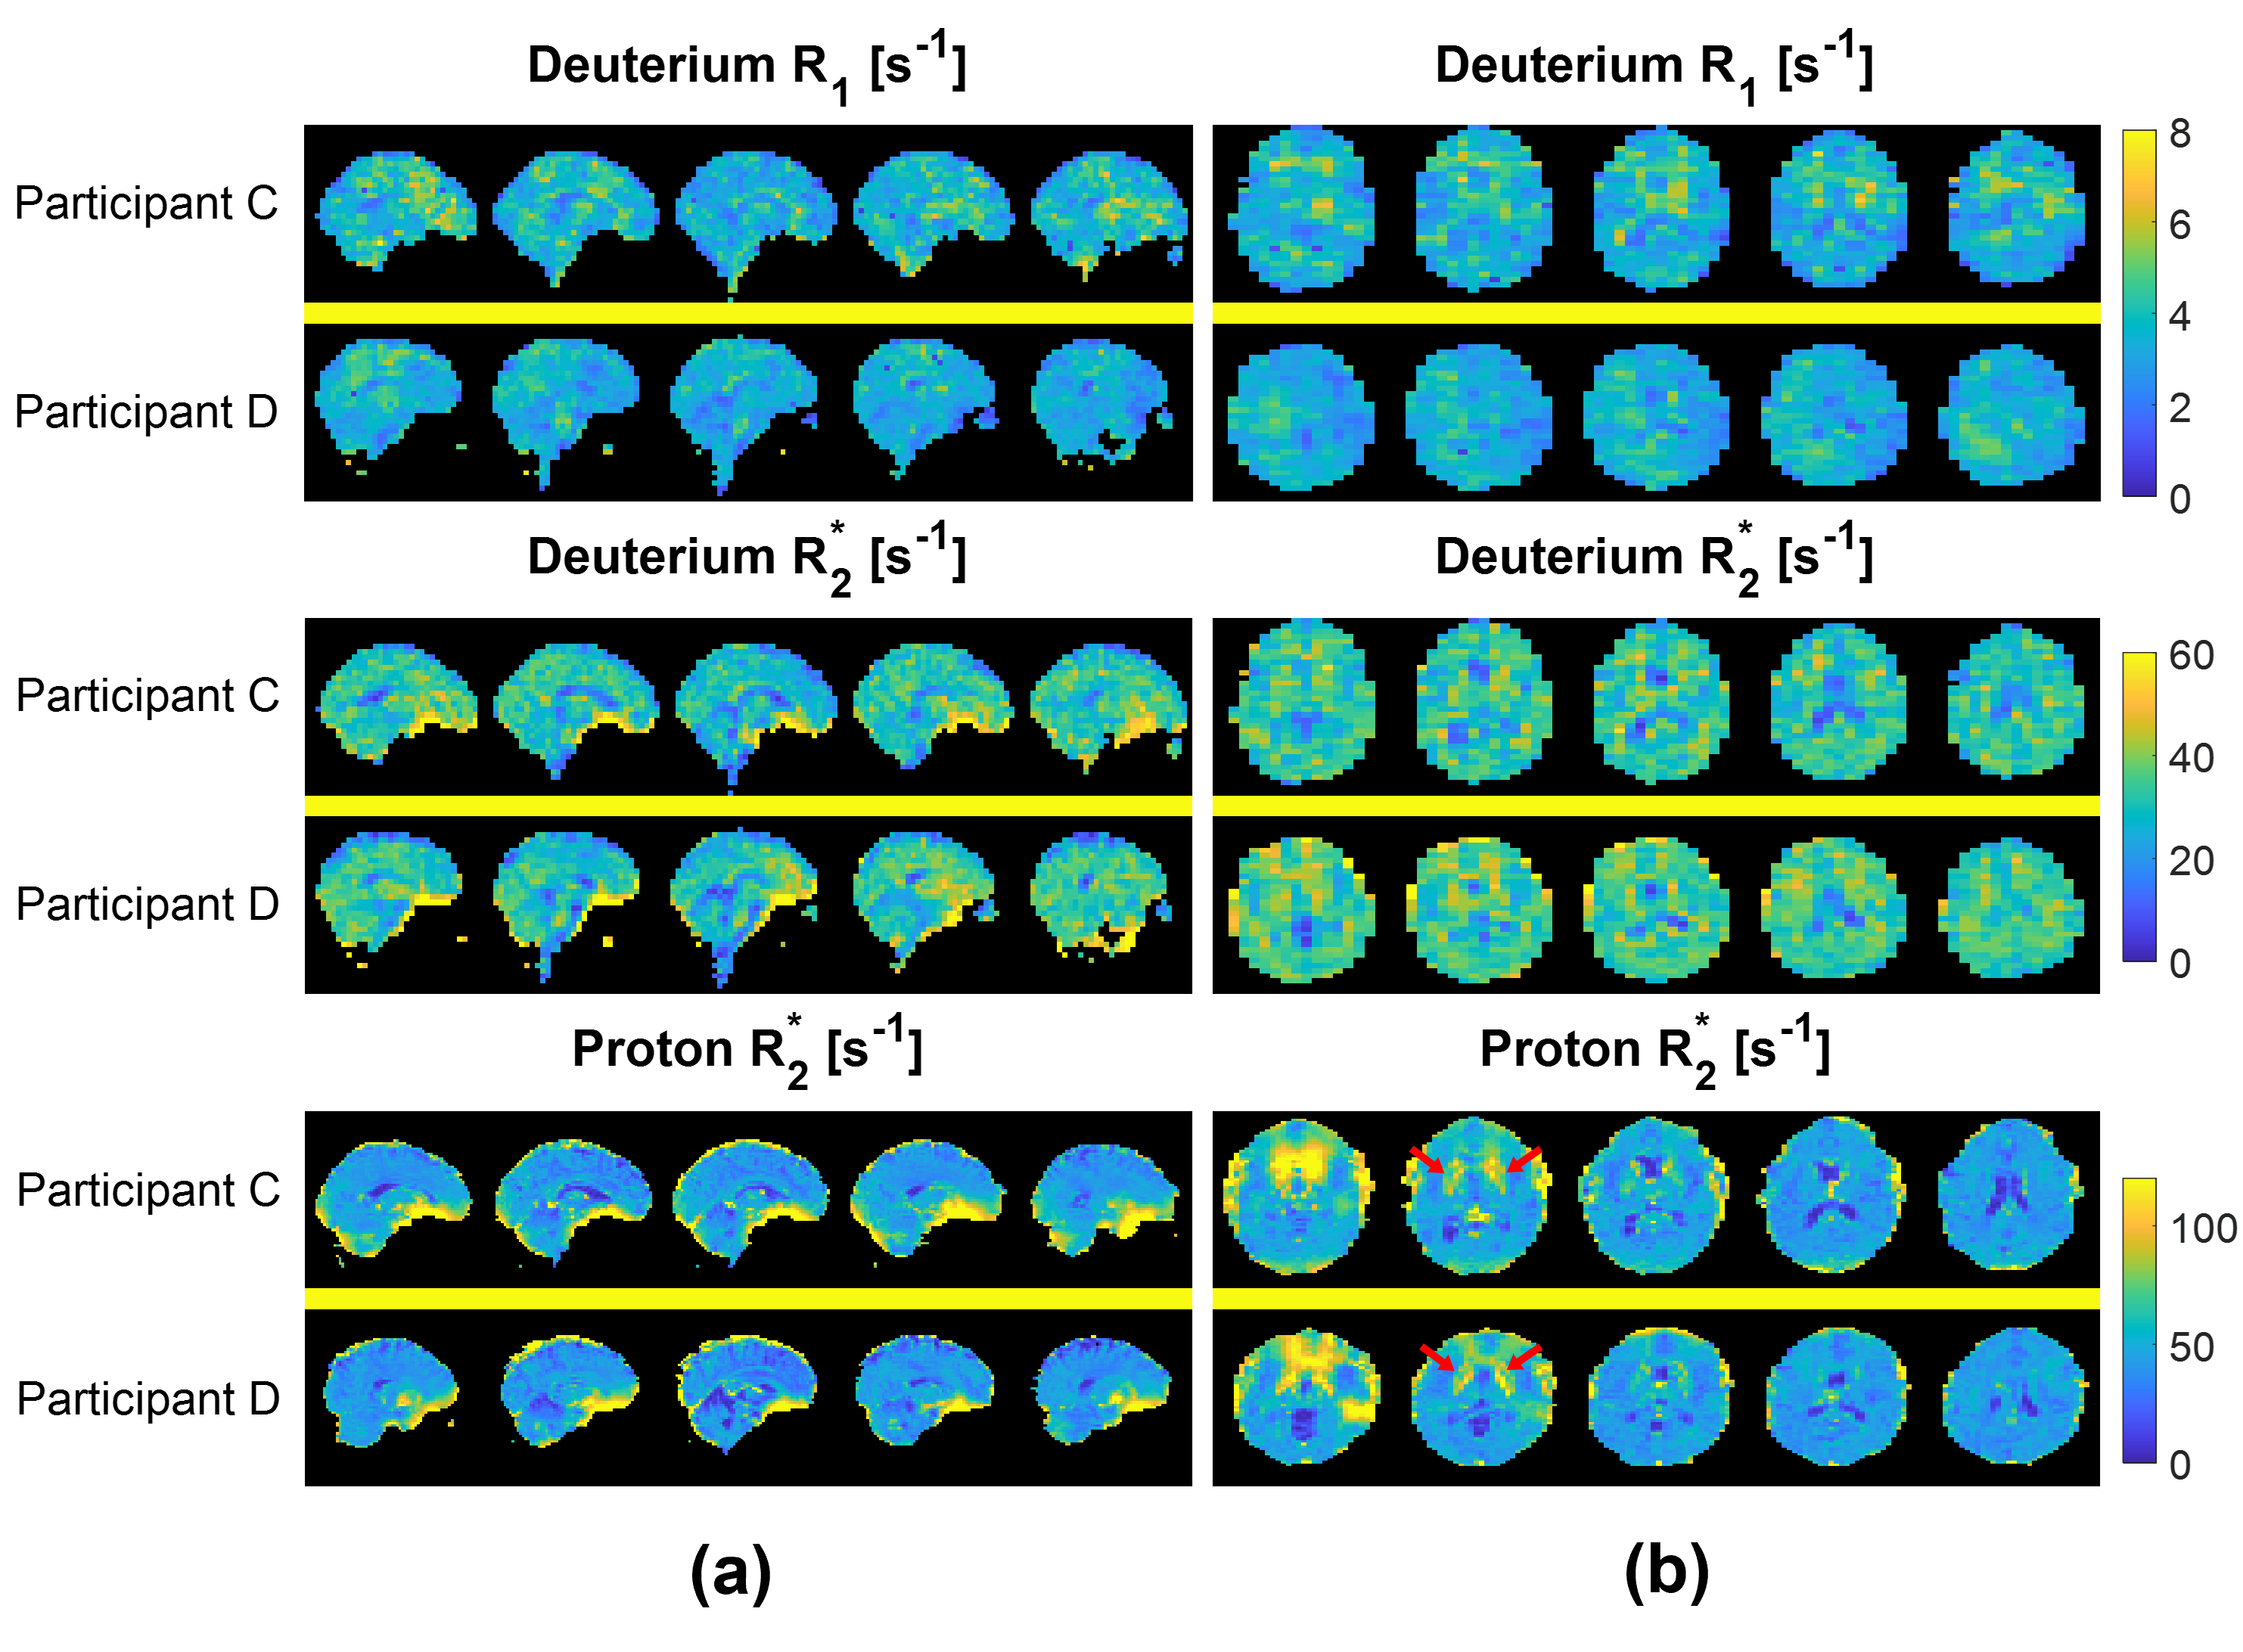
\includegraphics[width=1\textwidth]{Figures/D2O/R1_R2.png}
    \caption{\textit{$^2$H R$_2^*$ and R$_1$ maps are shown along with $^1$H R$_2^*$ maps in sagittal (a) and axial (b) format. Maps show five central slices from Participants C and D. Relaxation maps were calculated from MEGE data equivalent to that displayed in Fig. \ref{fig:D2O:TR_TE}. The elevated R$_2^*$ in iron-rich deep GM structures is evident in the lower slices of the $^1$H maps (red arrows), but is not seen in the $^2$H maps. The images shown have a reduced FOV of 204 × 204 mm$^2$.}}
    \label{fig:D2O:R1_R2}
\end{figure}

\begin{figure}
    \centering
    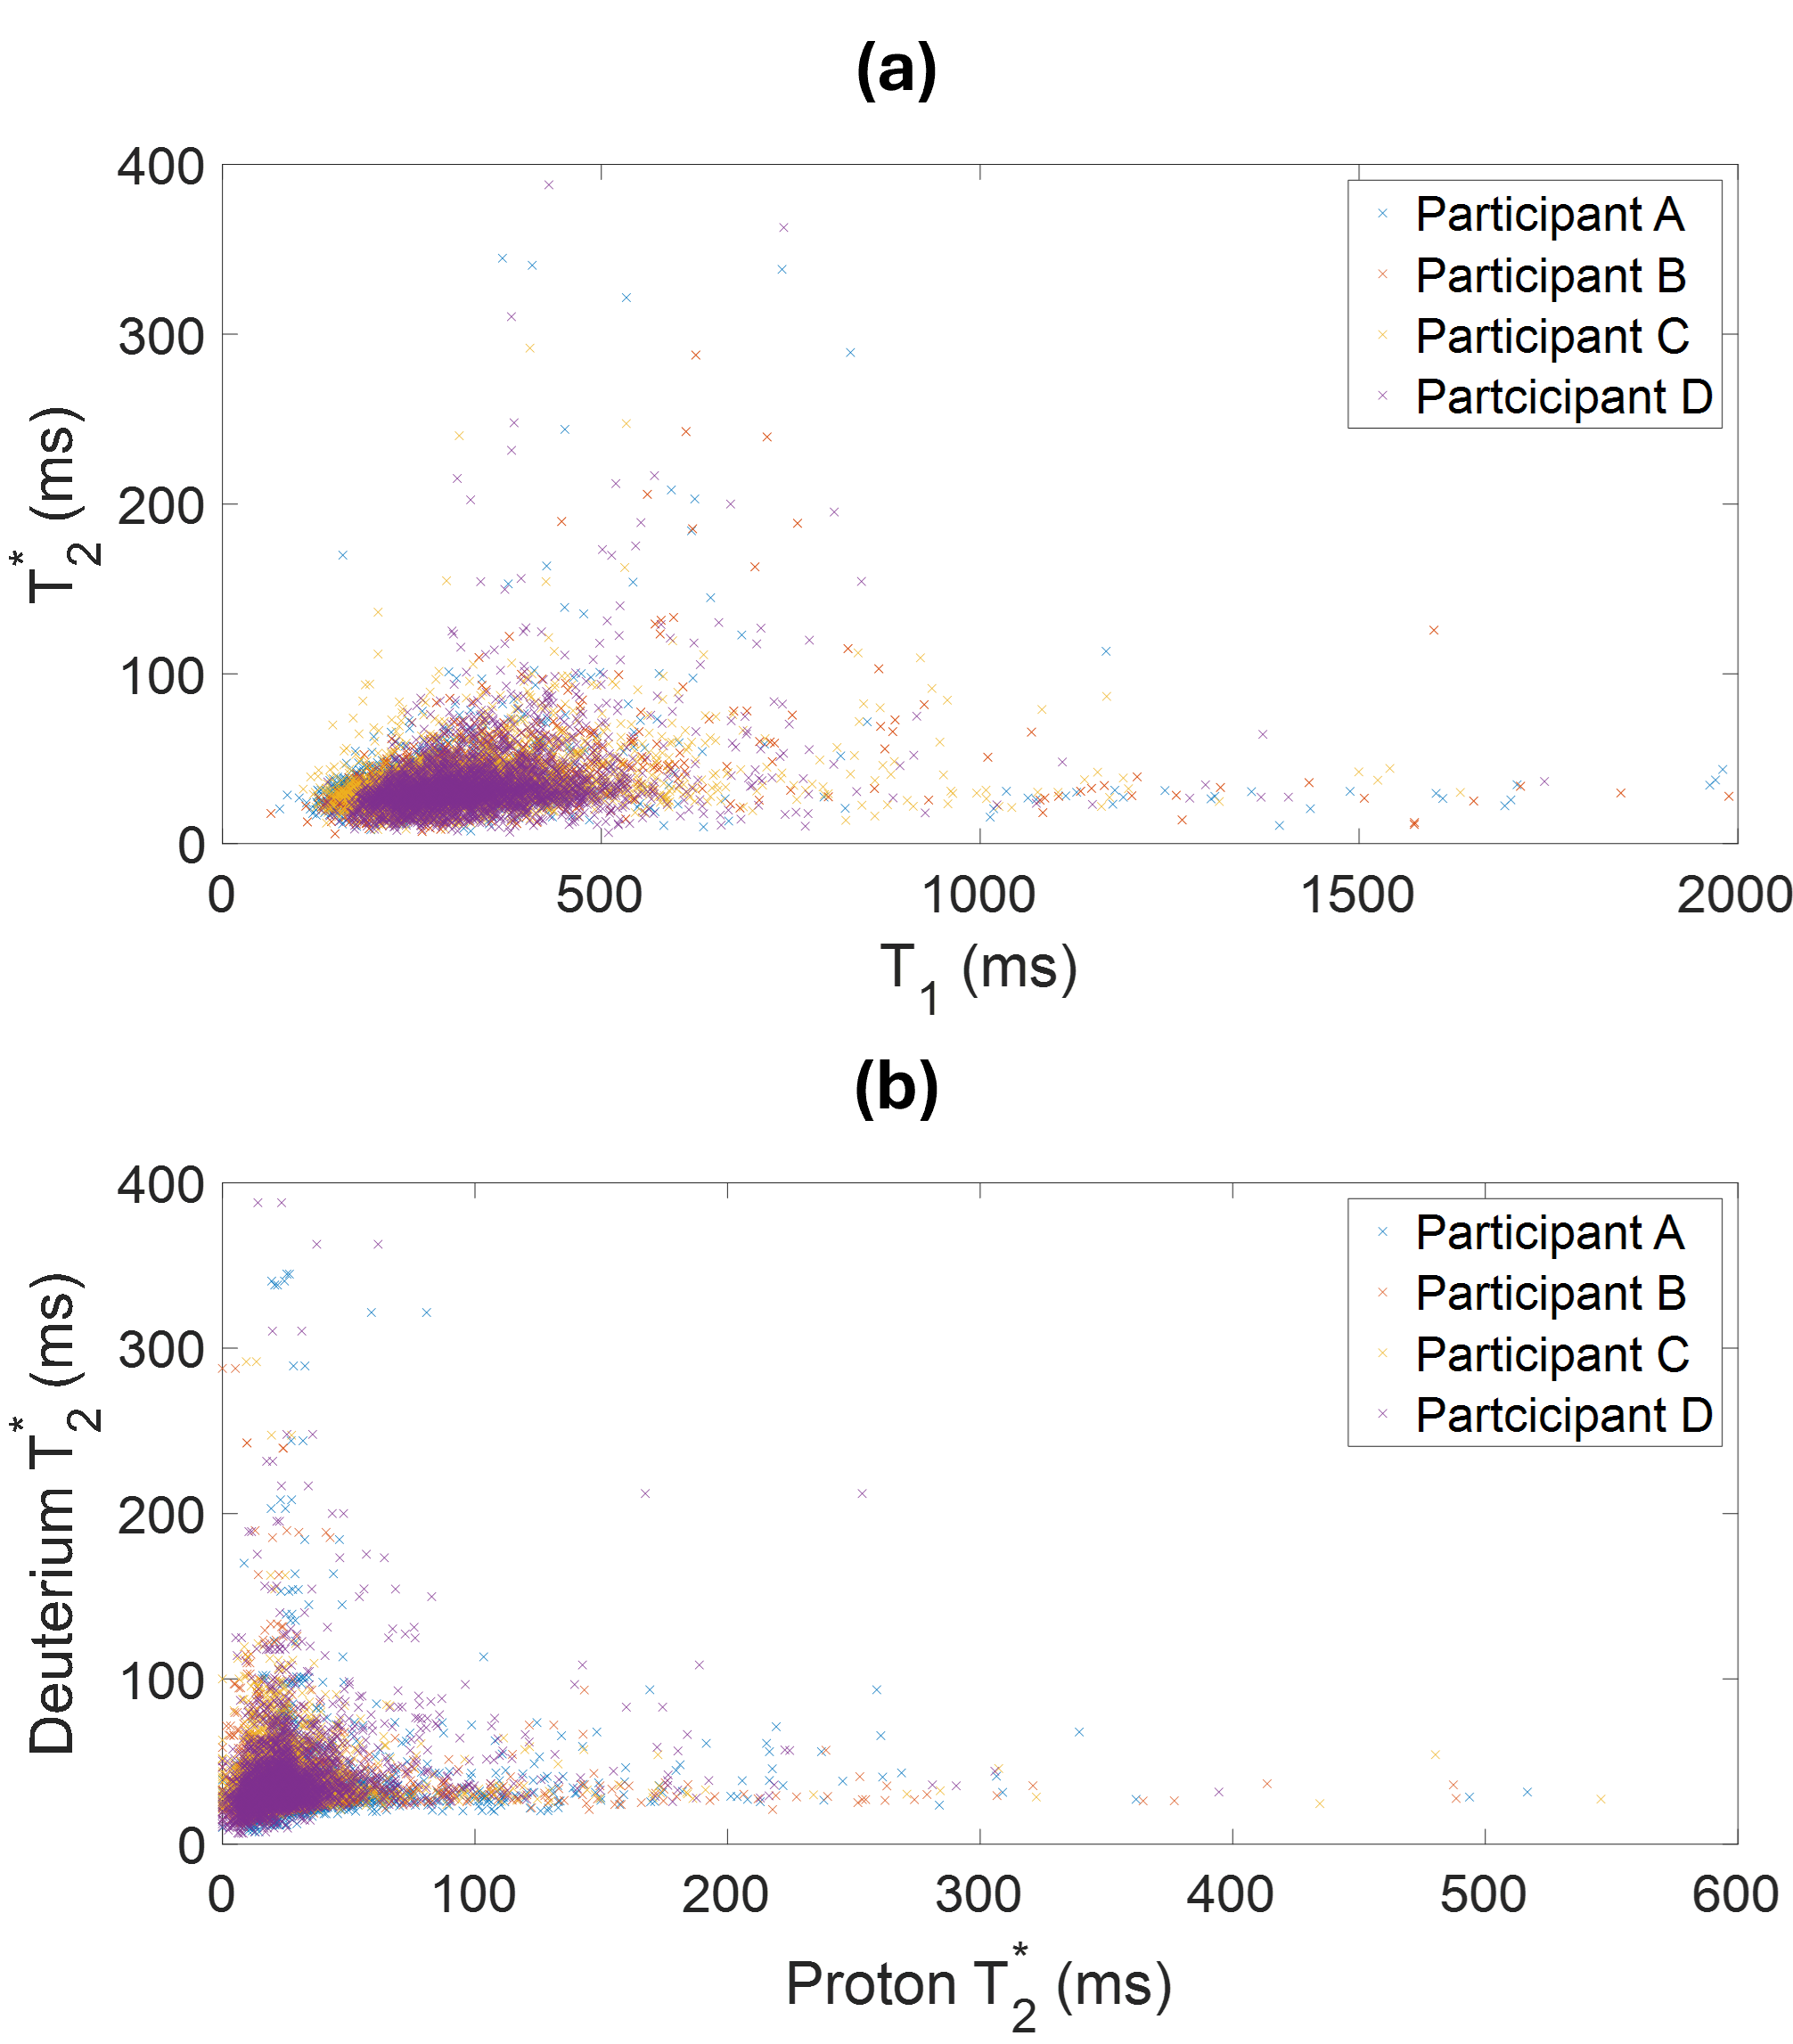
\includegraphics[width=1\linewidth]{Figures/D2O/Scatter.png}
    \caption{\textit{Scatter plots of the voxelwise deuterium T$_1$ and T$_2^*$ relaxation times (a) and the voxelwise proton and deuterium T$_2^*$ relaxation times (b).}}
    \label{fig:D2O:scatter}
\end{figure}

% Attempt to create overleaf table, data is too big for fontsize
% \noindent
% \begin{tabular}[H]{ |p{1cm}|p{0.5cm}||p{1cm}|p{1cm}|p{1cm}|p{1cm}|p{1cm}|p{1cm}|p{1cm}|p{1cm}|p{1cm}|  }
%     \hline
%     \multicolumn{2}{|c|}{} & \multicolumn{6}{|c|}{$^2$H relaxation times [ms]} & \multicolumn{3}{|c|}{$^1$H relaxation times [ms]} \\
%     \hline
%     \multicolumn{2}{|c|}{} & \multicolumn{2}{|c|}{CSF} & \multicolumn{2}{|c|}{GM} & \multicolumn{2}{|c|}{WM} & CSF & GM & WM \\
%     \hline
%     Subject & Visit & T$_1$ & T$_2^*$ & T$_1$ & T$_2^*$ & T$_1$ & T$_2^*$ & T$_2^*$ & T$_2^*$ & T$_2^*$ \\
%     \hline
%     A & 1 & 450 $\pm$ 200 & 110 $\pm$ 90 & 280 $\pm$ 100 & 32 $\pm$ 8 & 260 $\pm$ 100 & 30 $\pm$ 10 & 106 $\pm$ 90 & 26 $\pm$ 20 & 27 $\pm$ 20 \\
%     \hline
% \end{tabular}

\begin{table}[H]
    \centering
    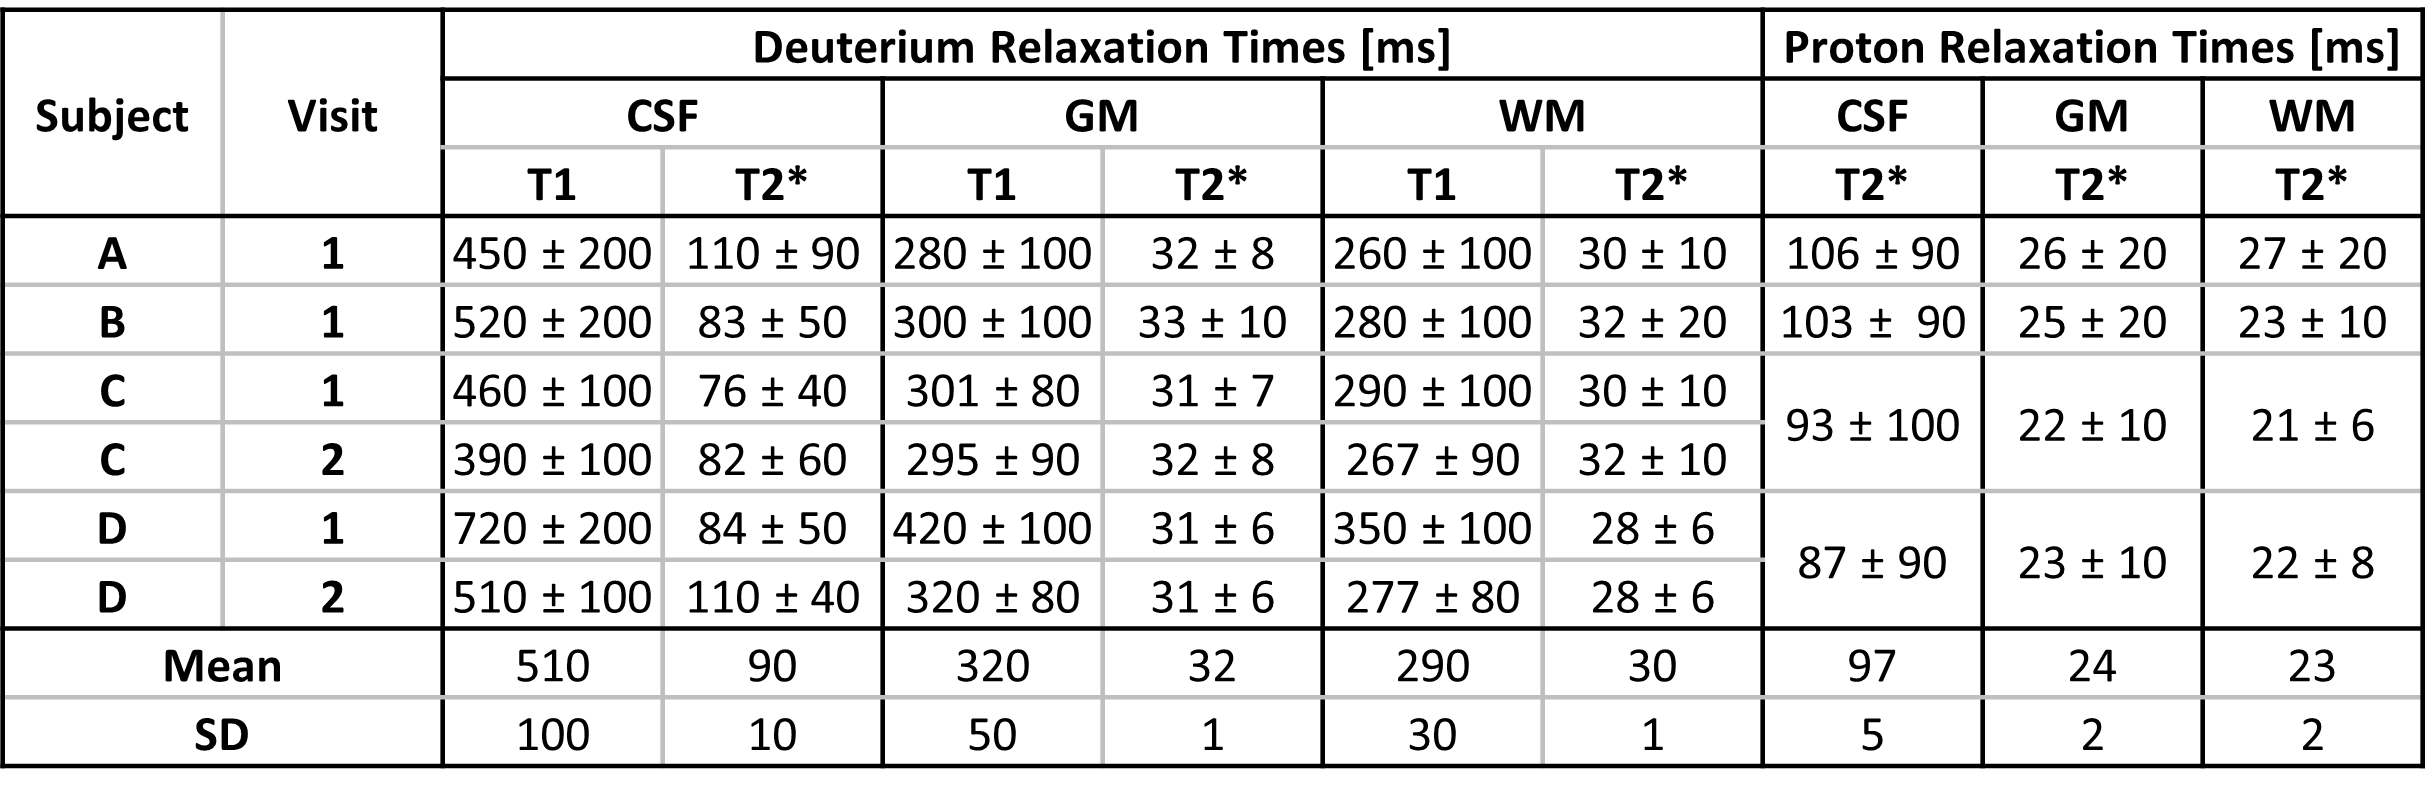
\includegraphics[width=1\textwidth]{Figures/D2O/R_Times.png}
    \caption{\textit{Average and SD of $^2$H (T$_2^*$ and T$_1$) and $^1$H (T$_2^*$) relaxation times in \ac{CSF}, \ac{GM}, and \ac{WM} for different participants and visits. These values were produced by averaging over segmented relaxation time maps, similar to those shown in Fig. \ref{fig:D2O:R1_R2}. Average values and standard deviations across participants are also shown.}}
    \label{fig:D2O:R_times}
\end{table}
 
\section{Discussion}

The results shown in Figs. \ref{fig:D2O:Sag_Full} and \ref{fig:D2O:Load} indicate that $^2$H images of 6 $\times$ 6 $\times$ 10 mm$^3$ voxel size with a useful \ac{SNR} can be acquired in $\sim$7.5 minutes at 7T with a head-sized bird-cage coil, when participants have been deuterium-enriched to $\sim$1.5\% concentration ($\sim$100 times \ac{NA}). After summing over echo times these images (Fig. \ref{fig:D2O:Load}) showed \ac{SNR} $\sim$16 in brain tissue in the steady-state condition (after 17 days of loading), the contrast in these images is dominated by T$_2^*$-weighting with the \ac{CSF} appearing hyperintense relative to grey and white matter.

The measured relaxation times were reasonably consistent across the six measurements (Table \ref{fig:D2O:R_times}), with \ac{CSF} having significantly higher T$_1$ and T$_2^*$ values than \ac{GM} or \ac{WM} (p $<$ 0.007 for two-sample t-test). The measured T$_1$ and T$_2^*$ values were consistently higher in \ac{GM} than in \ac{WM}, but the differences did not reach statistical significance (T$_1$: p = 0.21; T$_2^*$: p = 0.08). The relatively coarse resolution of the $^2$H images made it difficult to avoid the effects of partial voluming, particularly of \ac{CSF} and \ac{GM}, and the limited range of \ac{TE} and \ac{TR} values reduced the accuracy of measurement of the long T$_1$ and T$_2^*$ values in \ac{CSF}. The average values of the relaxation times are consistent with values reported from non-localised measurements of \ac{HDO} signals in human \cite{DeFeyter2018DeuteriumVivo,DeFeyter2021DeuteriumFuture,Ruhm2021DeuteriumResolution}, cat \cite{Ewy1988DeuteriumSitu} and rat  \cite{DeFeyter2018DeuteriumVivo,Lu2017QuantitativeSpectroscopy} brain.

Focusing on human brain measurements, De Feyter et al. \cite{DeFeyter2018DeuteriumVivo} reported HDO T$_1$ of 346 $\pm$ 5 ms at 4 T, while Ruhm et al. \cite{Ruhm2021DeuteriumResolution} measured 362 $\pm$ 6 ms at 9.4 T – values which lie between the values for \ac{CSF} (508 ms) and \ac{GM}/\ac{WM} (318/285 ms) measured here at 7 T. As expected, the measured $^2$H T$_1$-values are significantly shorter than the corresponding $^1$H values at 7 T \cite{Peters2007T27T}, due to the quadrupolar relaxation of $^2$H. The long T$_1$ of \ac{HDO} in \ac{CSF} relative to \ac{GM}/\ac{WM} will lead to greater saturation in the \ac{CSF} signal in short \ac{CSI} measurements used for \ac{DMI} (for example Ruhm et al. used TR = 155 ms \cite{Ruhm2021DeuteriumResolution}) which needs to be considered when quantifying signals from other $^2$H-labelled metabolites using \ac{NA} \ac{HDO} signals. Bi-exponential T$_2$ decay was previously identified at 4 T \cite{DeFeyter2018DeuteriumVivo} and 7 T \cite{Roig2022Deuterium7T} using non-localised spin echo measurements: at 7 T  large (small) pools were found to have relaxation times of 29 $\pm$ 1 (412 $\pm$ 40) ms, respectively \cite{Roig2022Deuterium7T}, consistent with our identification of short and long T$_2^*$ values in \ac{GM}/\ac{WM} (32/30 ms) and \ac{CSF} (90 ms). 

The \ac{TE}-summed \ac{MEGE} images in Figs. \ref{fig:D2O:Sag_Full} and \ref{fig:D2O:Load} show contrast that is dominated by T$_2^*$-weighting, with the \ac{CSF} appearing hyperintense relative to grey and white matter, as is the case in T$_2^*$-weighted $^1$H images. A notable difference between the $^1$H and $^2$H R$_2^*$ maps (Fig. \ref{fig:D2O:R1_R2}) is that deep \ac{GM} structures which appear with elevated R$_2^*$ in $^1$H maps due to their high iron content \cite{Peters2007T27T} do not appear hyperintense in the $^2$H maps. This is a consequence of the dominance of quadrupolar, rather than dipolar, relaxation in the case of $^2$H. The $^1$H R$_2^*$ maps also show larger regions of hyperintensity near the frontal sinuses due to the greater field-inhomogeneity-related intra-voxel dephasing resulting from the higher $\gamma$ of $^1$H. Signals from structures outside the brain (apart from the eyeball) are only evident in the $^2$H images acquired with the shortest \ac{TE} (Fig. \ref{fig:D2O:TR_TE}) most likely because of the very short T$_2^*$ of \ac{HDO} in muscle \cite{Gursan2022ResidualMuscle,Damion2021NaturalT}.

Both the imaging and spectroscopy results shown in Figs. \ref{fig:D2O:Bulk} and \ref{fig:D2O:ROI_Graph} show that changes in \ac{HDO} concentration on the order 0.1\% can be readily monitored and tracked, with spectroscopy data being obtained in one minute. At an estimated concentration of 0.5\% $^2$H, the ratio of signal to background noise varied from $\sim$2.7 (brain) to $\sim$3.1 (\ac{SC}) and these values increased approximately linearly with concentration as expected (Fig. \ref{fig:D2O:ROI_Graph}) to steady state levels over the 8-hour loading period. The normalised values here are not normalised for flip-angle here. The concentrations estimated from the $^2$H spectra are in reasonably good agreement with the values calculated from the cumulative \ac{D$_2$O} dose and body mass (Fig. \ref{fig:D2O:Bulk}). 

In addition, the signal amplitudes measured from \ac{ROI}s in the brain have similar time-courses maintaining relatively constant ratios, dictated mainly by differences in T$_2^*$-weighting and water fraction in the different brain regions (Fig. \ref{fig:D2O:ROI_Graph}). It is also important to note that as subject C stopped loading (after $\sim$350 minutes) a reduction in the rate of increase in $^2$H concentration is evident in both Figs. \ref{fig:D2O:Bulk} and \ref{fig:D2O:ROI_Graph}, on the scale of minutes. This implies that the $^2$H MR measurements are robust and that the dispersal kinetics of deuterium following oral ingestion of \ac{D$_2$O} are rapid throughout the body on the timescale of the measurements. This is consistent with previous measurements based on blood sampling which indicate that the half-life of absorption into blood is around 12 min, with similar time constants for dispersal into other body water compartments \cite{Davies2001RapidWater,Peronnet2012PharmacokineticHumans}. 

In our experiments the participants came out of the magnet bore between measurements, leading to the potential for changes in signal intensity due to variation of the slice position. Nevertheless the $^2$H signals tracked the monotonically increasing dose and the values measured at maximum dose were similar to those measured 17 days later during the steady state loading period. Although both participants had approximately the same weight and target \ac{D$_2$O} dose, Participant B was only able to ingest 600 ml during the initial loading. The deuterium concentration measured from Participant A was consequently higher at the end of the loading period. The rest of participant B’s loading was completed over the following four days, along with the daily 50 ml top-up and similar concentrations were measured from the two participants in the steady state (Fig. \ref{fig:D2O:Bulk}). The tracked GCMS analysis of saliva samples during loading is given in this figure. The saliva samples do not follow the deuterium concentration by body-weight estimates as closely as the spectroscopy measurements as well as being much more variable  The GCMS measurements of the saliva at the end of the loading was 1.51\% $\pm$ 0.09\%, and 1.53\% $\pm$ 0.17\%, respectively for participants A and B. 

Rapid increases in body water enrichment can lead to feelings of dizziness and nausea. These symptoms can occur at relatively low enrichments while equilibrium has not yet been achieved, and are thought to result from temporary effects on the vestibular system due to density changes in the semi-circular canals of the inner ear \cite{Money1974HeavyAlcohol}. The rapid loading was required for the parallel study, but a more gradual increase in heavy water uptake could be used for future MR-loading experiments to minimise these effects. 
%This meant that some of the subjects were unable to finish the rapid loading in the first day. This can be seen in Figs. \ref{fig:D2O:Load}, \ref{fig:D2O:ROI_Graph} and \ref{fig:D2O:Bulk} which is why Participant B was only able to ingest 600 ml out of the 800 ml, despite having approximately the same weight as Participant A, and why the rate of \ac{D$_2$O} loading was slowed. This effect has caused previous participants to withdraw, no female participant was able to complete the initial loading in the first day. There are numerous reasons that could explain this behavior, one of which being possible less body water \% meaning the estimated dosage was too high. This could be explained by reports of women having a higher motion sickness susceptibility \cite{Flanagan2005SexSickness.}, this difference has also been made aware during spaceflight as female crew-members report post-flight vestibular instability symptoms more frequently than men \cite{Reschke2014EffectsSystems}. One possible explanation is the sexual dimorphism in the size of structures in the vestibular system, as many structures have been found to be larger in men \cite{Sato2016Computer-AidedApparatus}. However, no firm explanation on the cause of this apparent motion sickness has been made, it is unknown whether it is affecting this study.  

\section{Conclusion}

$^2$H MR measurements at 7T have been successfully used to track the increase in concentration of $^2$H in brain during \ac{D$_2$O} loading to 100 times \ac{NA}, in four human participants. Gradient echo images with an \ac{SNR} of 16 and a voxel volume of 0.36 ml could be acquired in 7.5 minutes. $^2$H T$_1$ and T$_2^*$ relaxation times from water in \ac{GM}, \ac{WM} and \ac{CSF} have also been measured at 7T. These relaxation times can be applied in research protocols using the \ac{NA} $^2$H signal from water for calibration and concentration calculations. This lays the ground work for further studies involving ingested \ac{D$_2$O} in order to measure lipid turnover in Chapter \ref{Chap:Lipid}. In future work we aim to track uptake from a single \ac{D$_2$O} dose on a shorter time scale, using faster, interleaved acquisition of $^2$H images and spectra. 